% to compile: Shift+Alt+F1
\documentclass[a4paper,11pt]{article}%,twocolumn
%% packages

\usepackage{blindtext} % needed for creating dummy text passages
%\usepackage{ngerman} % needed for German default language
\usepackage{amsmath} % needed for command eqref
\usepackage{amssymb} % needed for math fonts
\usepackage[colorlinks=true,breaklinks]{hyperref} % needed for creating hyperlinks in the document, the option colorlinks=true gets rid of the awful boxes, breaklinks breaks lonkg links (list of figures), and ngerman sets everything for german as default hyperlinks language
\usepackage[hyphenbreaks]{breakurl} % ben�tigt f�r das Brechen von URLs in Literaturreferenzen, hyphenbreaks auch bei links, die �ber eine Seite gehen (mit hyphenation).
\usepackage{xcolor}
\definecolor{c1}{rgb}{0,0,1} % blue
\definecolor{c2}{rgb}{0,0.3,0.9} % light blue
\definecolor{c3}{rgb}{0.3,0,0.9} % red blue
\hypersetup{
    linkcolor={c1}, % internal links
    citecolor={c2}, % citations
    urlcolor={c3} % external links/urls
}
%\usepackage{cite} % needed for cite
\usepackage[square,authoryear]{natbib} % needed for cite and abbrvnat bibliography style
\usepackage[nottoc]{tocbibind} % needed for displaying bibliography and other in the table of contents
\usepackage{graphicx} % needed for \includegraphics 
\usepackage{longtable} % needed for long tables over pages
\usepackage{bigstrut} % needed for the command \bigstrut
\usepackage{enumerate} % needed for some options in enumerate
%\usepackage{todonotes} % needed for todos
\usepackage{makeidx} % needed for creating an index
\makeindex
\usepackage{gensymb}
%\usepackage{url}
\usepackage{xurl}
\usepackage{psfrag}
\usepackage{multirow}
\usepackage{subfigure}

\usepackage{algpseudocode}
\usepackage{float}
%\usepackage{minted}
\usepackage{tcolorbox}
\usepackage{menukeys}
\usepackage[
width=.8\textwidth,
justification=centering]{caption}
\usepackage{xcolor}
\usepackage{pstricks}
\usepackage{acronym}
%% page settings

\usepackage[top=20mm, bottom=20mm,left=20mm,right=20mm]{geometry} % needed for page border settings
\parindent=0mm % for space of first line of new text block
\sloppy % for writing with hyphenless justification (tries to)
\hyphenation{} % use hyphenation of tolerance parametershttp://www.jr-x.de/publikationen/latex/tipps/zeilenumbruch.html
\hyphenpenalty=10000
\exhyphenpenalty=10000
\usepackage{fancyhdr} % needed for head and foot options
%% my macros

%% Text fomats
\newcommand{\tbi}[1]{\textbf{\textit{#1}}}

% IEEE naming convention
%\renewcommand{\figurename}{Fig.}

% custom counter for shell scripts
\newcounter{shellcounter}
% \newcounter{myexample}% preamble
\newtcolorbox[
use counter=shellcounter,
number format=\Alph]{shell}[2][]{%
	colback=blue!5!white,
	colframe=blue!75!white,
	fonttitle=\bfseries,
	title= {\sc Shell \thetcbcounter}: #2,#1}


\newcounter{outputcounter}
\newtcolorbox[
use counter=outputcounter,
number format=\Roman]{result}[2][]{%
	colback=green!5!white,
	colframe=green!75!black,
	fonttitle=\bfseries,
	title= {\sc Result box \thetcbcounter}: #2,#1}


\begin{document}
\begin{titlepage}
\center % Center everything on the page

%-------------------------------------------------------------------------------------
%	HEADING SECTIONS
%------------------------------------------------------------------------------------
\textbf{\large Department of Electronic and Telecommunication Engineering}\\[0.5cm]
\textbf{\Large University of Moratuwa, Sri Lanka}\\[1cm]
\textbf{\large EN4603 - Digital IC Design}\\[2cm]

\includegraphics[width=0.3\textwidth]{figures/uomlogo}\\[2cm]

	
%-------------------------------------------------------------------------------------
%	TITLE SECTION
%------------------------------------------------------------------------------------
\textbf{\Huge Laboratory Experiment 1 \\RTL Synthesis }\\[0.2cm]
\textbf{\Large Laboratory Report}\\[3cm]


%----------------------------------------------------------------------------------------
%	MEMBERS SECTION
%----------------------------------------------------------------------------------------


\vfill

\textbf{\large Submitted by}\\[0.5cm]

\textbf{\large Submitted by}\\[2mm]
\begin{minipage}{0.3\textwidth}
	\begin{flushleft}
		{\large C.S.Pallikkonda}\\[2mm]
		{\large R.M.A.S.Rathnayake }\\[2mm]
		{\large B.P.Thalagala }\\[2mm]		
		
	\end{flushleft}
\end{minipage}
\hspace{2mm}
\begin{minipage}{0.2\textwidth}
	\begin{flushright}
		{\large 180441C }\\[2mm]
		{\large 180534N }\\[2mm]
		{\large 180631J }\\[2mm]

	\end{flushright}
\end{minipage}\\[1cm]

	
	
	
%----------------------------------------------------------------------------------------
%	DATE SECTION
%----------------------------------------------------------------------------------------

\textbf{\large Submitted on}\\[0.5cm]
\textbf{\Large \today} % Date, change the \today to a set date if you want to be precise

%----------------------------------------------------------------------------------------

\vfill % Fill the rest of the page with whitespace

\end{titlepage}

\pagebreak

\tableofcontents
\vfill
\textit{\textbf{Note:}}\\
\textit{All the materials related to the report can also be found at \url{https://github.com/bimalka98/Digital-IC-Design}}

\pagebreak
\listoffigures
\listoftables
\section*{List of Abbreviations}
\addcontentsline{toc}{section}{List of Abbreviations}
\begin{acronym}
	\acro{asic}[ASIC]{Application Specific Integrated Circuit}
	\acro{atpg}[ATPG]{Automatic Test Pattern Generation}
	
	\acro{def}[DEF]{Design Exchange Format}
	\acro{dft}[DFT]{Design For Testability}
		
	\acro{gpdk}[GPDK]{Generic Process Design Kit}
		
	\acro{hdl}[HDL]{Hardware Description Language}
	
	\acro{ic}[IC]{Integrated Circuit}
		
	\acro{rtl}[RTL]{Register-Transfer Level}
	\acro{rx}[RX]{Receiver}
		
	\acro{tcl}[TCL]{Tool Command Language}
	\acro{tx}[TX]{Transmitter}
	
	\acro{uart}[UART]{Universal Asynchronous Receiver Transmitter}
	
\end{acronym}






\pagebreak
\section{Introduction}

\subsection{Practical}
In this practical, you will be using \textit{Cadence Innovus} to place and route the design you synthesized in Laboratory Experiment 2. As inputs to Innovus, you will provide,

\begin{enumerate}
	\item Source Verilog files
	\item Technology libraries provided by the fabrication plant (here, $45~nm$ educational \ac{gpdk} given by Cadence) : {\tt (.lib, .lef, .tch)}
	
	\begin{itemize}
		\item Library Timing (.lib) files specify timing (cell delay, cell transition time, setup and hold time requirement) and power characteristics of standard cells. Slow and fast libraries 	characterize standard cells with maximum and minimum signal delays, which could occur from process variations.

		\item Tch files are binary files that accurately characterize library elements, that include  capacitance and resistance.
		
		\item Library Exchange Format (LEF) specify design rules, metal capacitances, layer information…etc.
	\end{itemize}
	
	\item Multi Mode Multi Corner file (.view)
	\item Constraints file (.sdc)
	\item Scan \ac{def} file (.scandef)
\end{enumerate}

and will obtain the GDSII file as output, which is an industry standard format for exchanging \ac{ic} layout data. You will then analyze, compare, and comment on the placement, cell count, congestion etc. of the design at various stages of the place and route design flow.

\subsection{Place \& Route}

Place \& route is the final step in the IC design flow before fabrication. As the name implies, this step comprises of two main tasks – placement and routing.\\

In placement, the IC designer decides where to place all the elements of the design. In addition to placing cells, this step involves making initial decisions about the aspect ratio and utilization factors (core utilization / cell utilization).\\

Then, in the routing step, the designer makes the physical interconnects between the placed elements. This step comprises of three main stages: (1) Power Routing: routing of VDD and GND nets, (2) Clock Tree Synthesis: re-synthesizing of clock nets based on cell placement in order to balance clock skew throughout the design and minimize insertion delay, and (3) Signal Routing: routing of all other nets.\\

\pagebreak
The general design flow for place \& Route, which we will be following in this laboratory experiment, is shown in Figure \ref{fig:flow}.

\begin{figure}[h]
	\centering
	\fbox{
		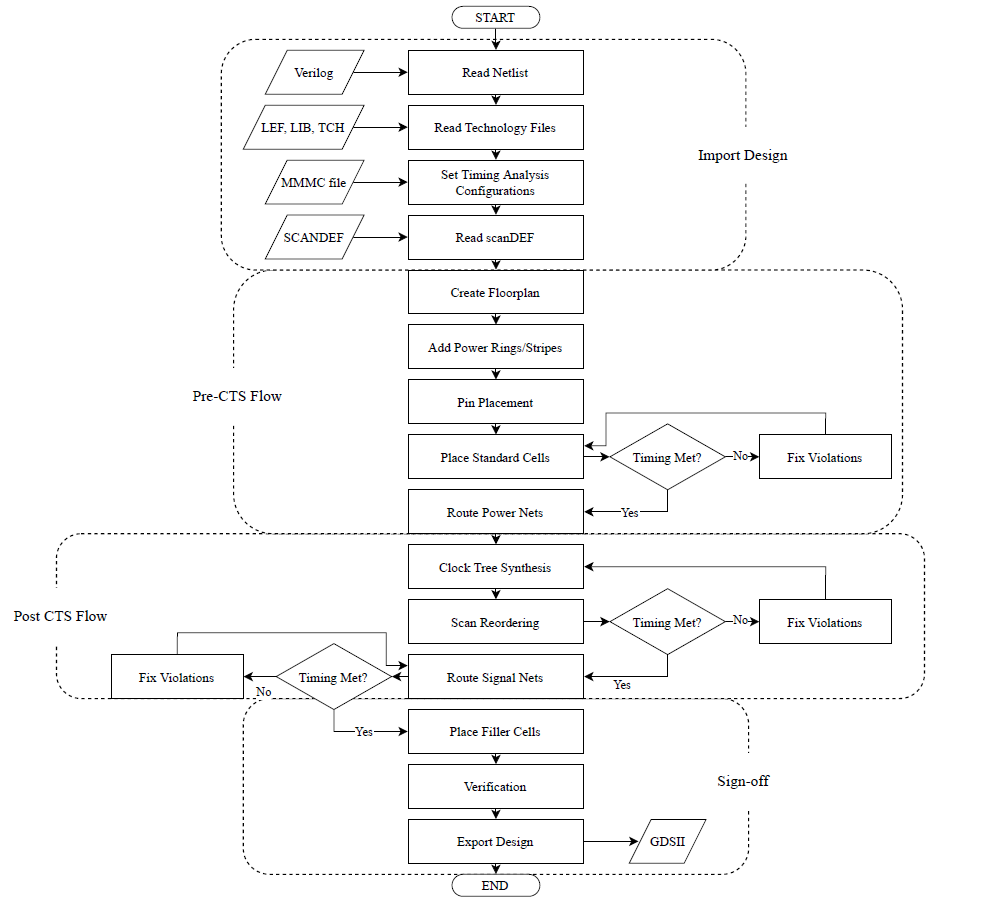
\includegraphics[width=0.95\linewidth]{figures/flow}
	}
	\caption{The general design flow for place \& Route}
	\label{fig:flow}
\end{figure}

\pagebreak
\section{Using Innovus for Place and Route}
This section demonstrates the steps carried out at the `Step 3' in the Laboratory guide, with necessary illustrations.

\begin{enumerate}[1.)]
	\item Import the Design: this step loads the design according to the netlist, technology libraries, labels for power nets and the timing analysis configurations. Once the design is loaded an empty core in the design area of Innovus can be observed as shown in the Figure \ref{fig:innovus_1},  and it displays ``In Memory'' in the bottom right corner of Innovus.
	
	\begin{figure}[h]
		\centering
		\fbox{
			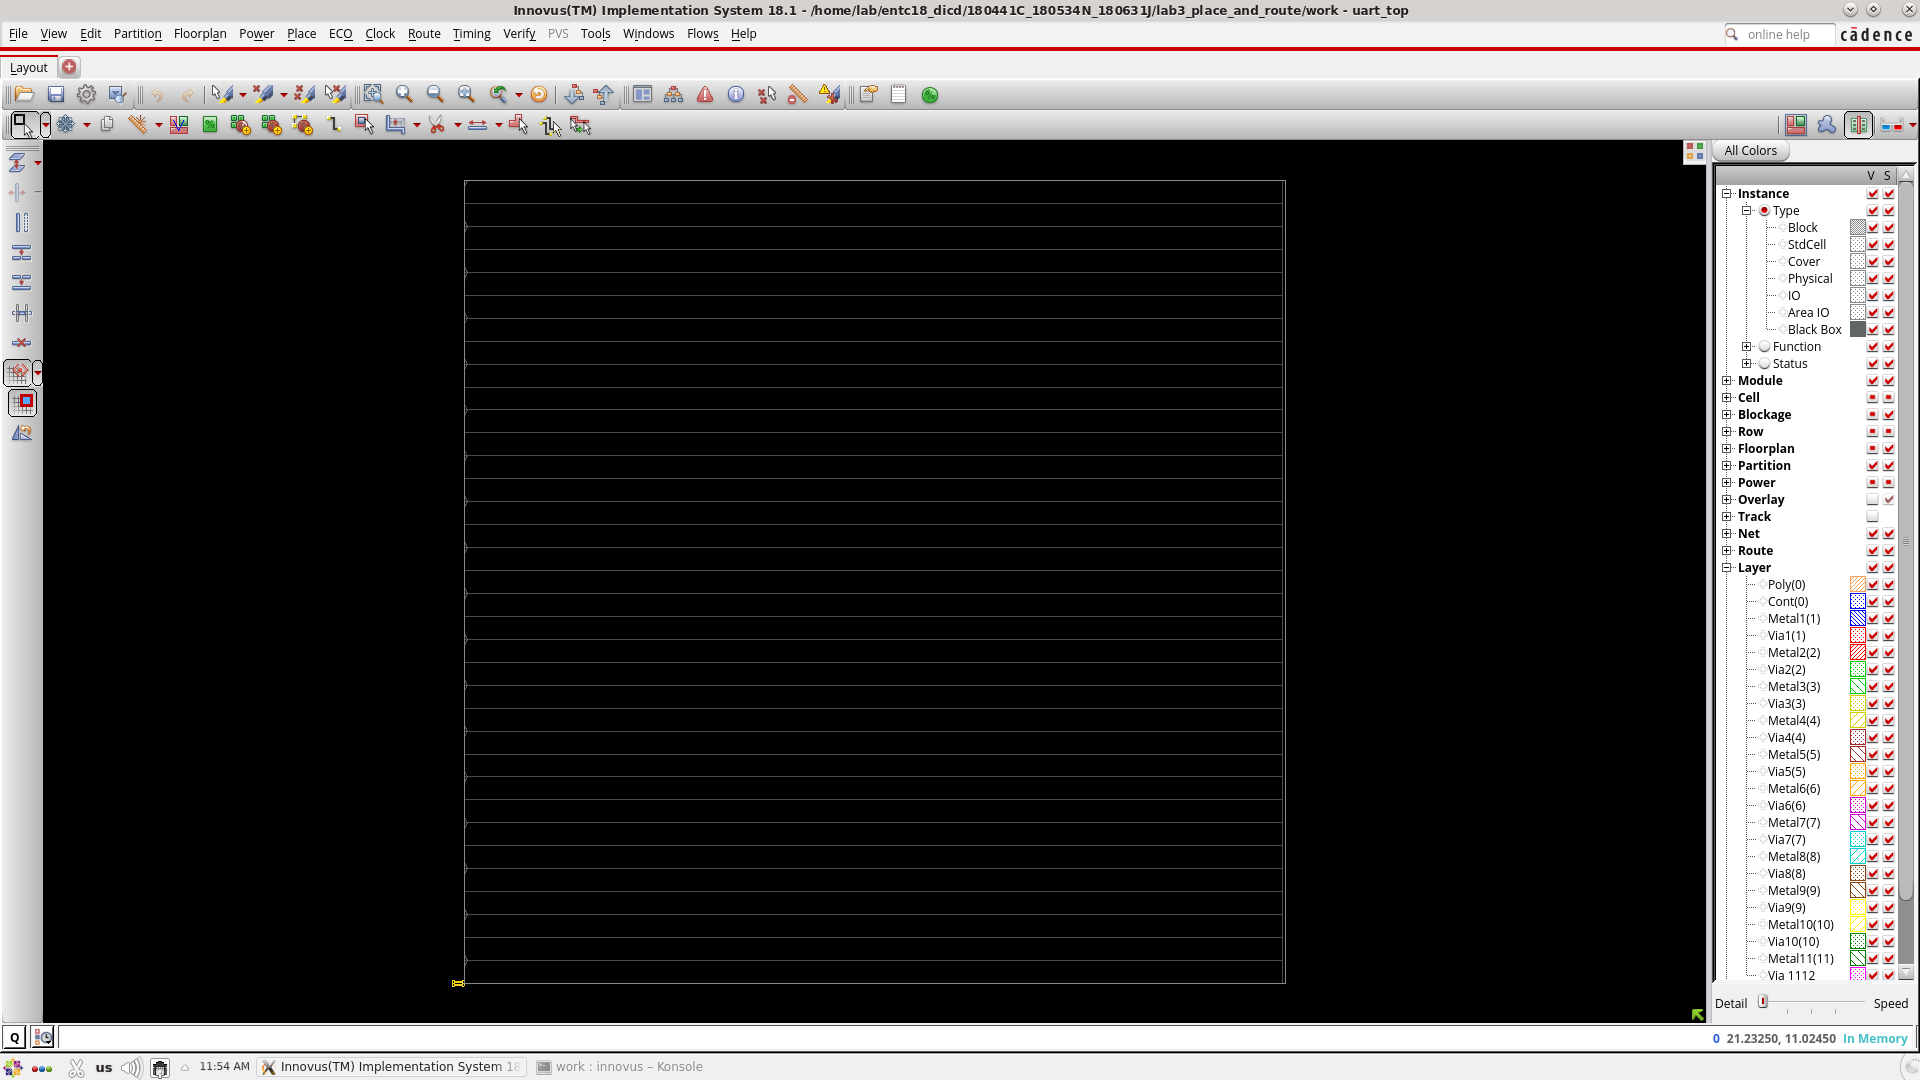
\includegraphics[width=0.95\linewidth]{figures/innovus_1.png}
		}
		\caption{Empty core in the design area of Innovus, when the design is loaded}
		\label{fig:innovus_1}
	\end{figure}
	
	
	\item  Read the scanDEF file: this file specifies the scan chains available in the design and to perform scan reordering later.
	
	\begin{figure}[h]
		\centering
		\fbox{
			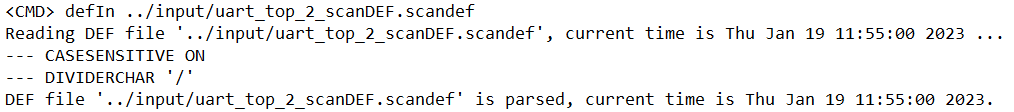
\includegraphics[width=0.95\linewidth]{figures/defIn}
		}
		\caption{Innovus log for reading the scan\ac{def} file}
		\label{fig:defIn}
	\end{figure}
	
	\item Set the design mode to 45nm process
	
	\begin{figure}[h]
		\centering
		\fbox{
			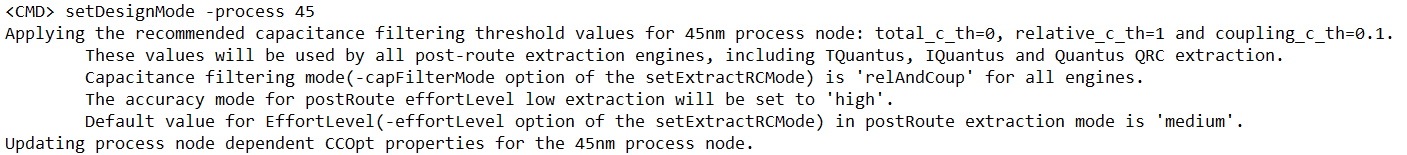
\includegraphics[width=0.95\linewidth]{figures/setDesignMode}
		}
		\caption{Innovus log for setting the design mode to 45nm process}
		\label{fig:setDesignMode}
	\end{figure}
	\pagebreak
	\item Specify floorplan: Set the \textit{Aspect Ratio} as 1.0 and \textit{Core Utilization} as 0.4.  Set core margins by core to \ac{io} boundary. Set a margin of 5 Microns to all sides from the core. This resulted in a floor plan shown in the Figure \ref{fig:innovus_2}.
	
	\begin{figure}[h]
	\centering
	\fbox{
		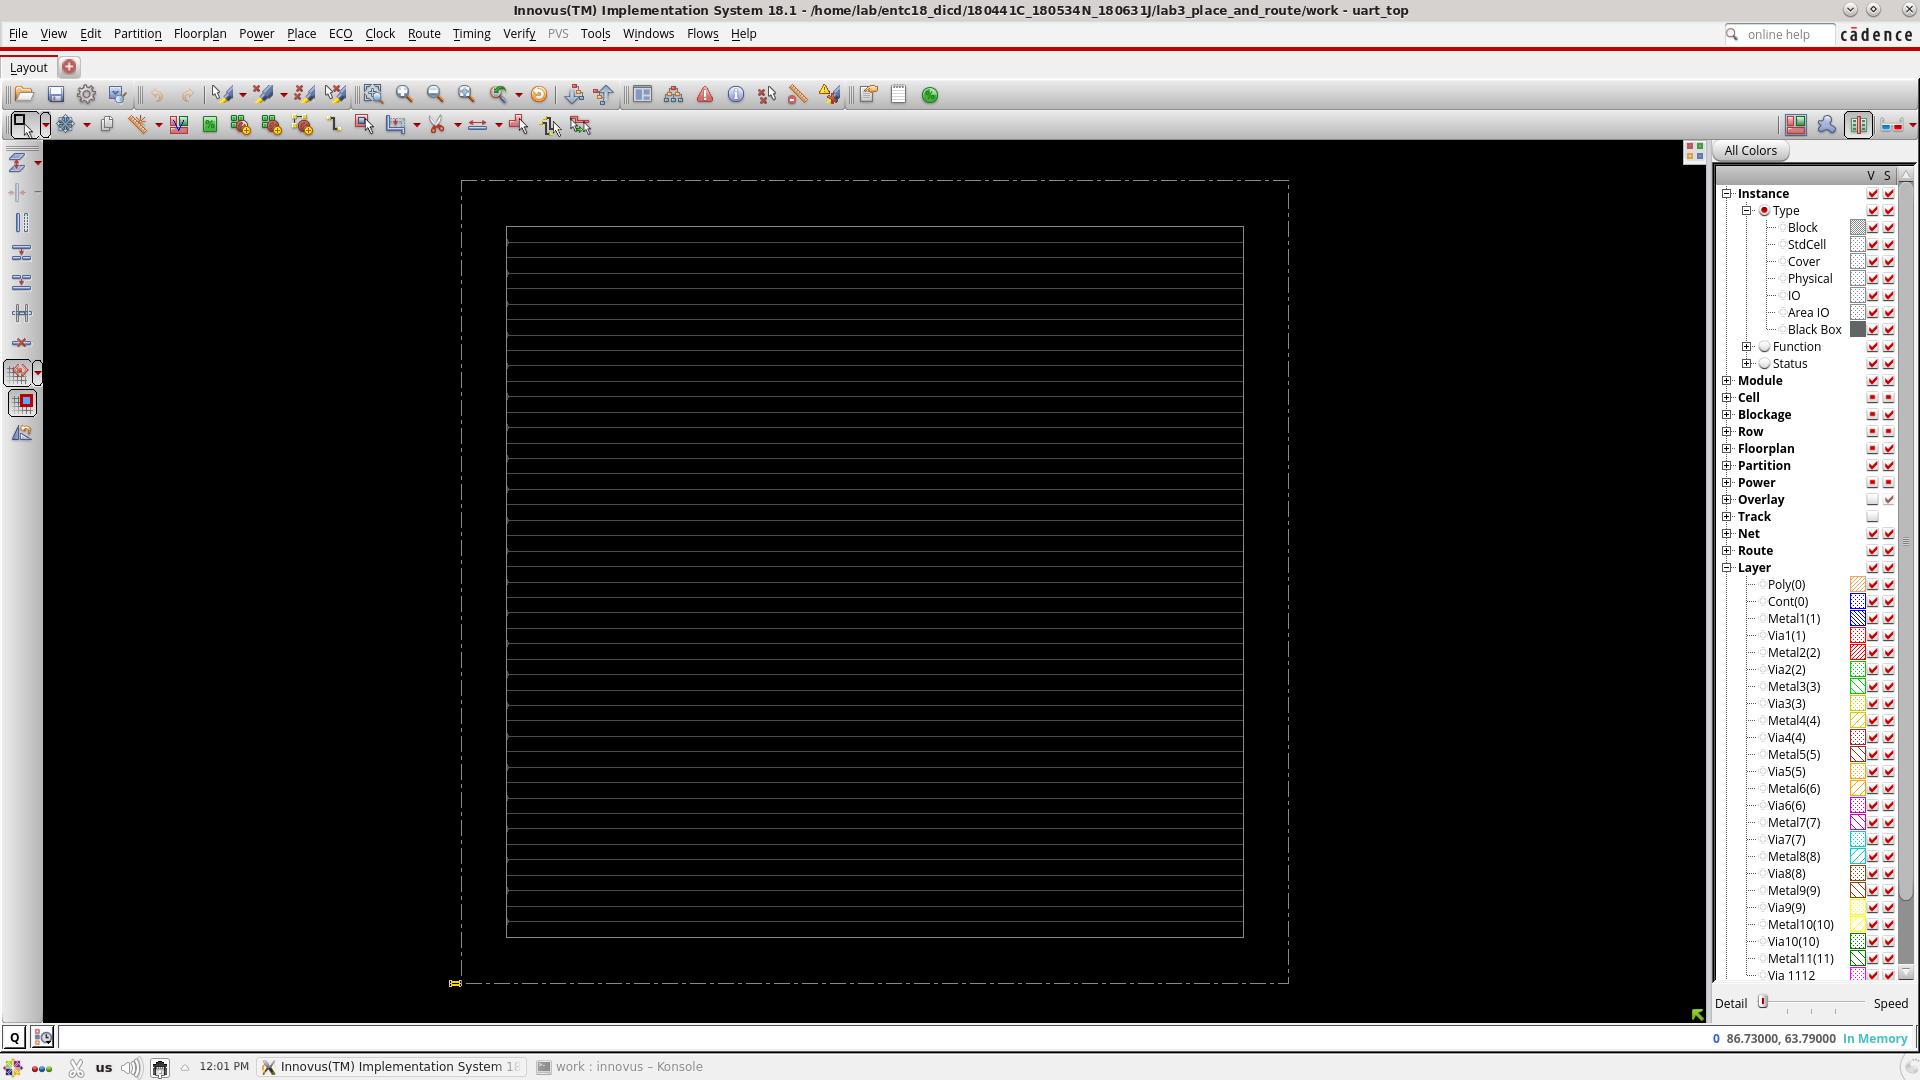
\includegraphics[width=0.9\linewidth]{figures/innovus_2.png}
	}
	\caption{Specified floorplan}
	\label{fig:innovus_2}
	\end{figure}
		
	\item Add power rings and power stripes:Metal 7 layer is used  for for horizontal power rings/stripes, while Metal 8  layer for vertical power rings/stripes.
	
	\begin{enumerate}[a.]
		\item  Power rings
		\begin{figure}[H]
			\centering
			\fbox{
				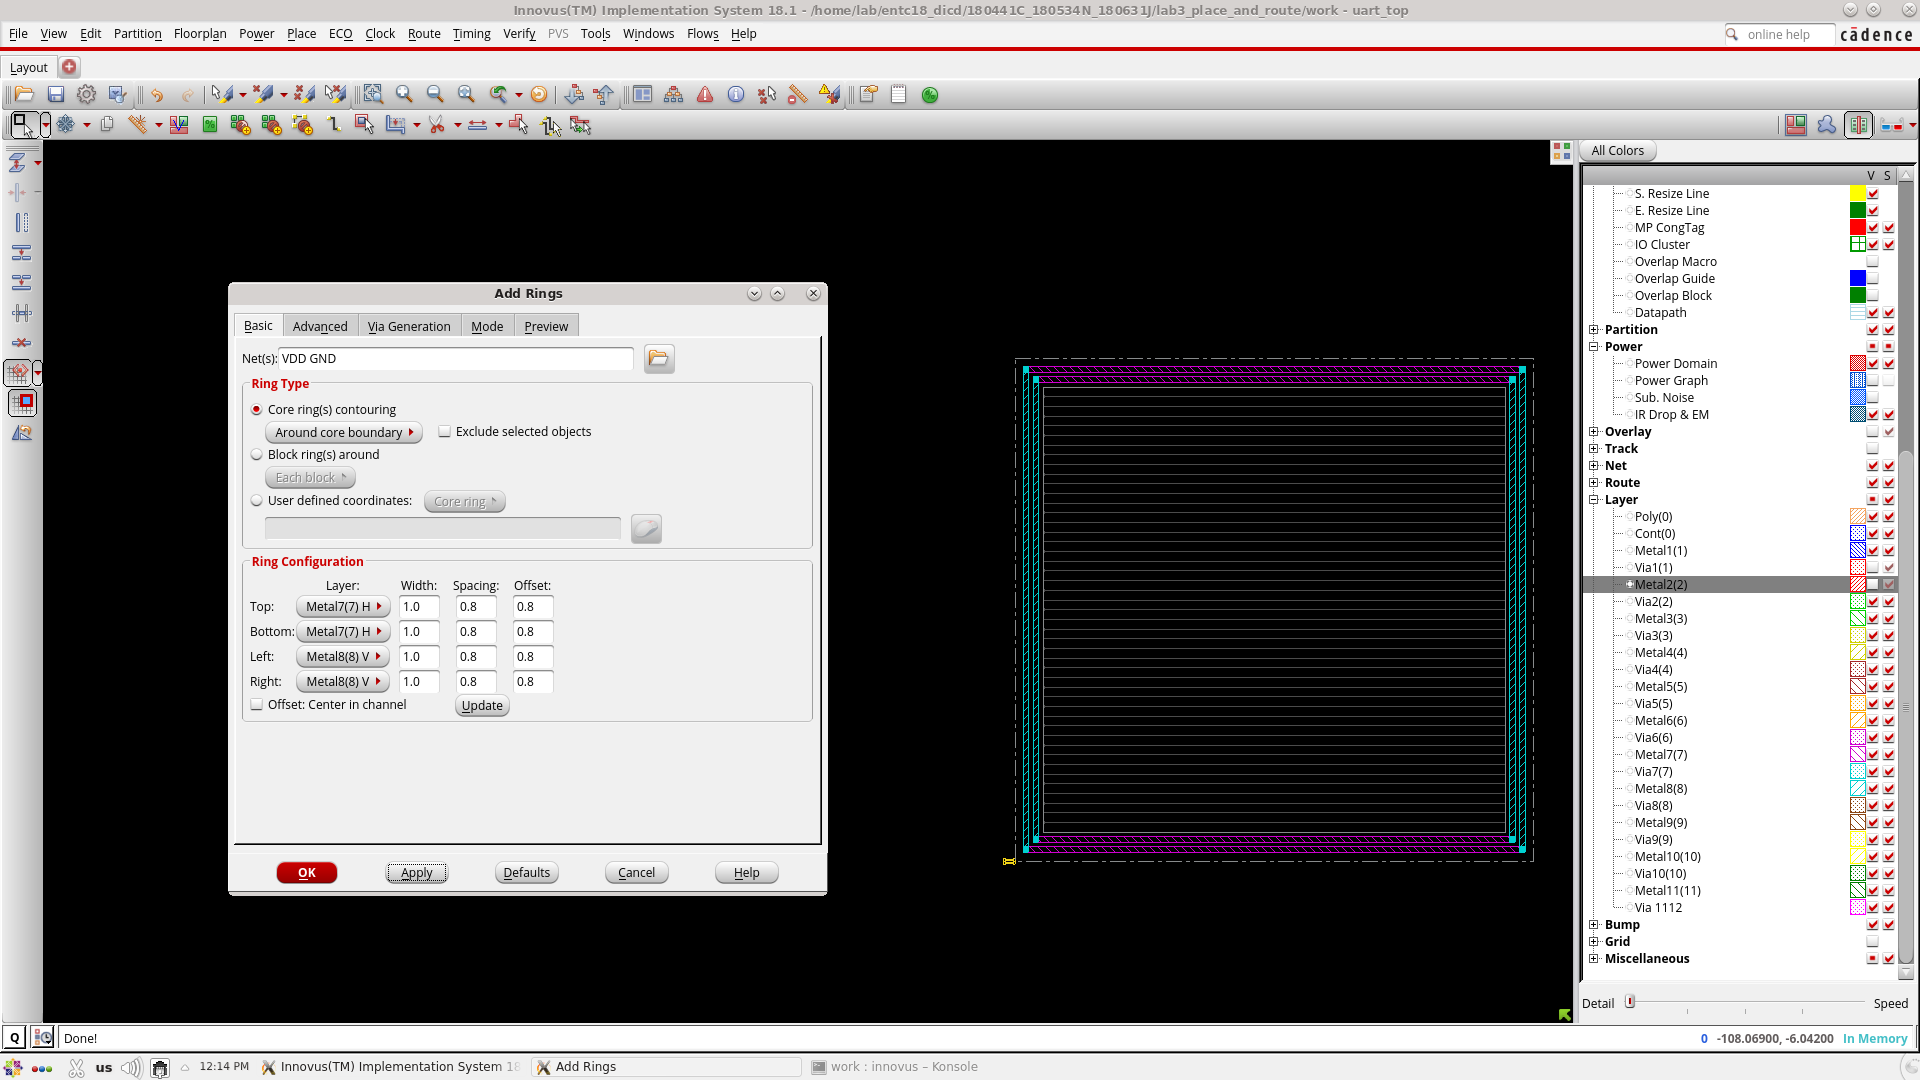
\includegraphics[width=0.9\linewidth]{figures/innovus_3_2.png}
			}
			\caption{Adding power rings}
			\label{fig:innovus_3_2}
		\end{figure}
		\pagebreak
		\item Horizontal power strips
		\begin{figure}[H]
			\centering
			\fbox{
				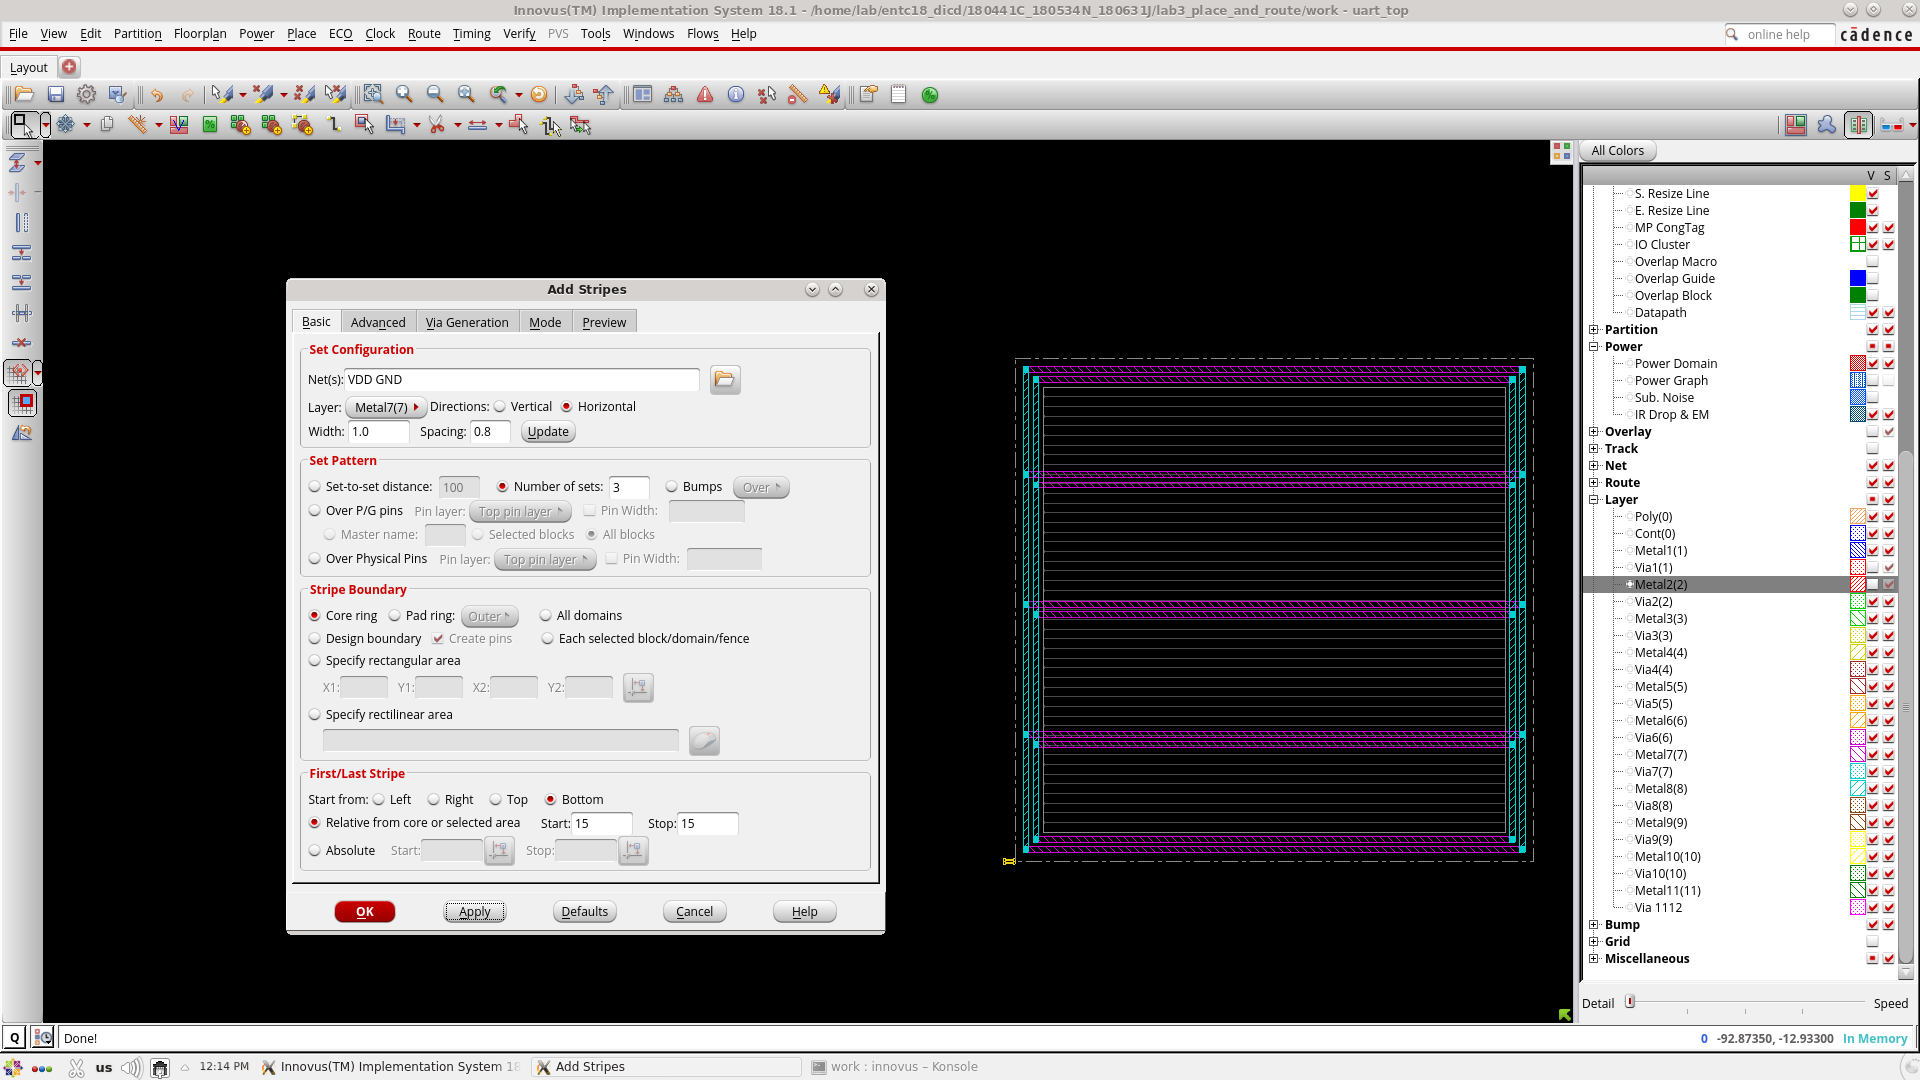
\includegraphics[width=0.9\linewidth]{figures/innovus_4_2.png}
			}
			\caption{Adding horizontal power strips}
			\label{fig:innovus_4_2}
		\end{figure}
		
		\item Vertical power strips
		\begin{figure}[H]
			\centering
			\fbox{
				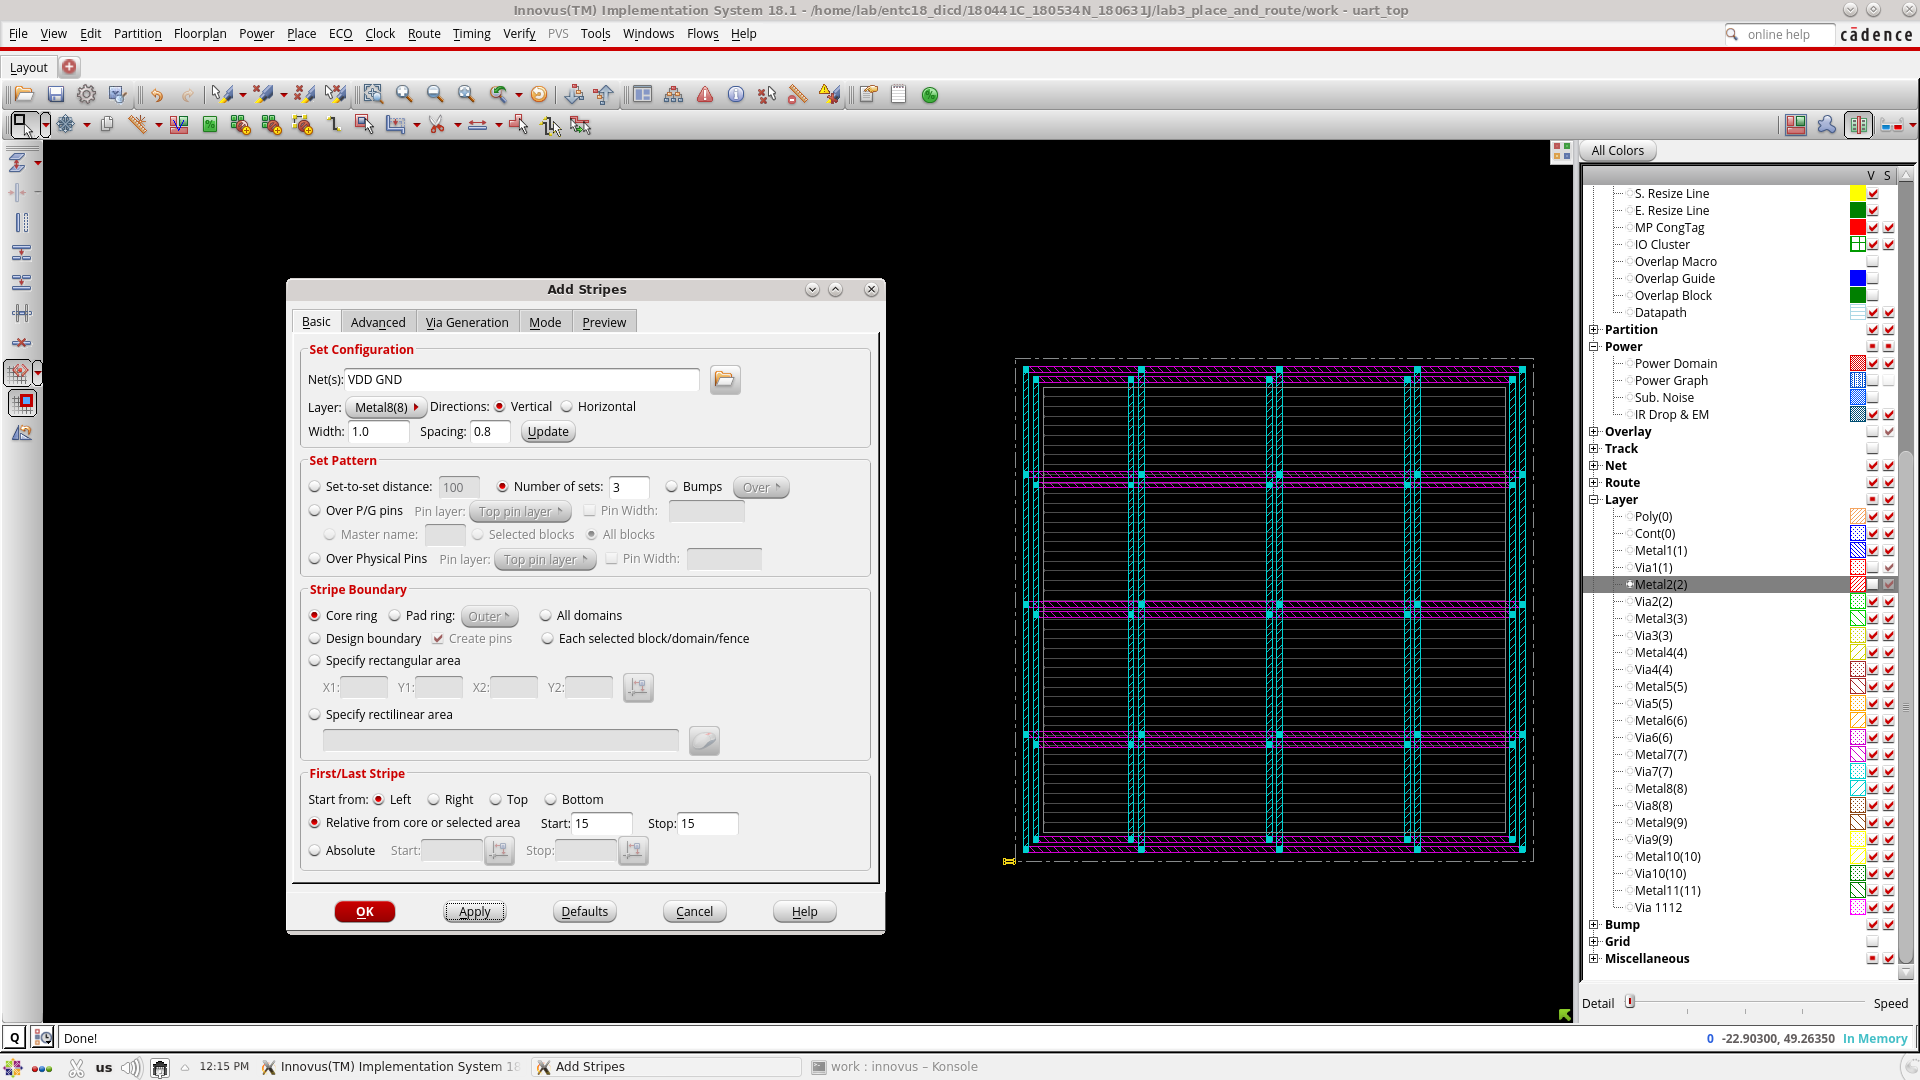
\includegraphics[width=0.9\linewidth]{figures/innovus_4_4.png}
			}
			\caption{Adding vertical power strips}
			\label{fig:innovus_4_4}
		\end{figure}	
	\end{enumerate}
	
	\pagebreak
	\item Pin Placement: assigns a set of pin to the \ac{io} boundary. By default the pins are set as \textit{SIGNAL} pins. However, we should change this attribute for the clock pins {\tt clk\_a} and {\tt clk\_b} to \textit{CLOCK}. Figure \ref{fig:innovus_6_1} illustrated the view of the floorplan after all the pins are assigned.
	
	\begin{figure}[H]
		\centering
		\fbox{
			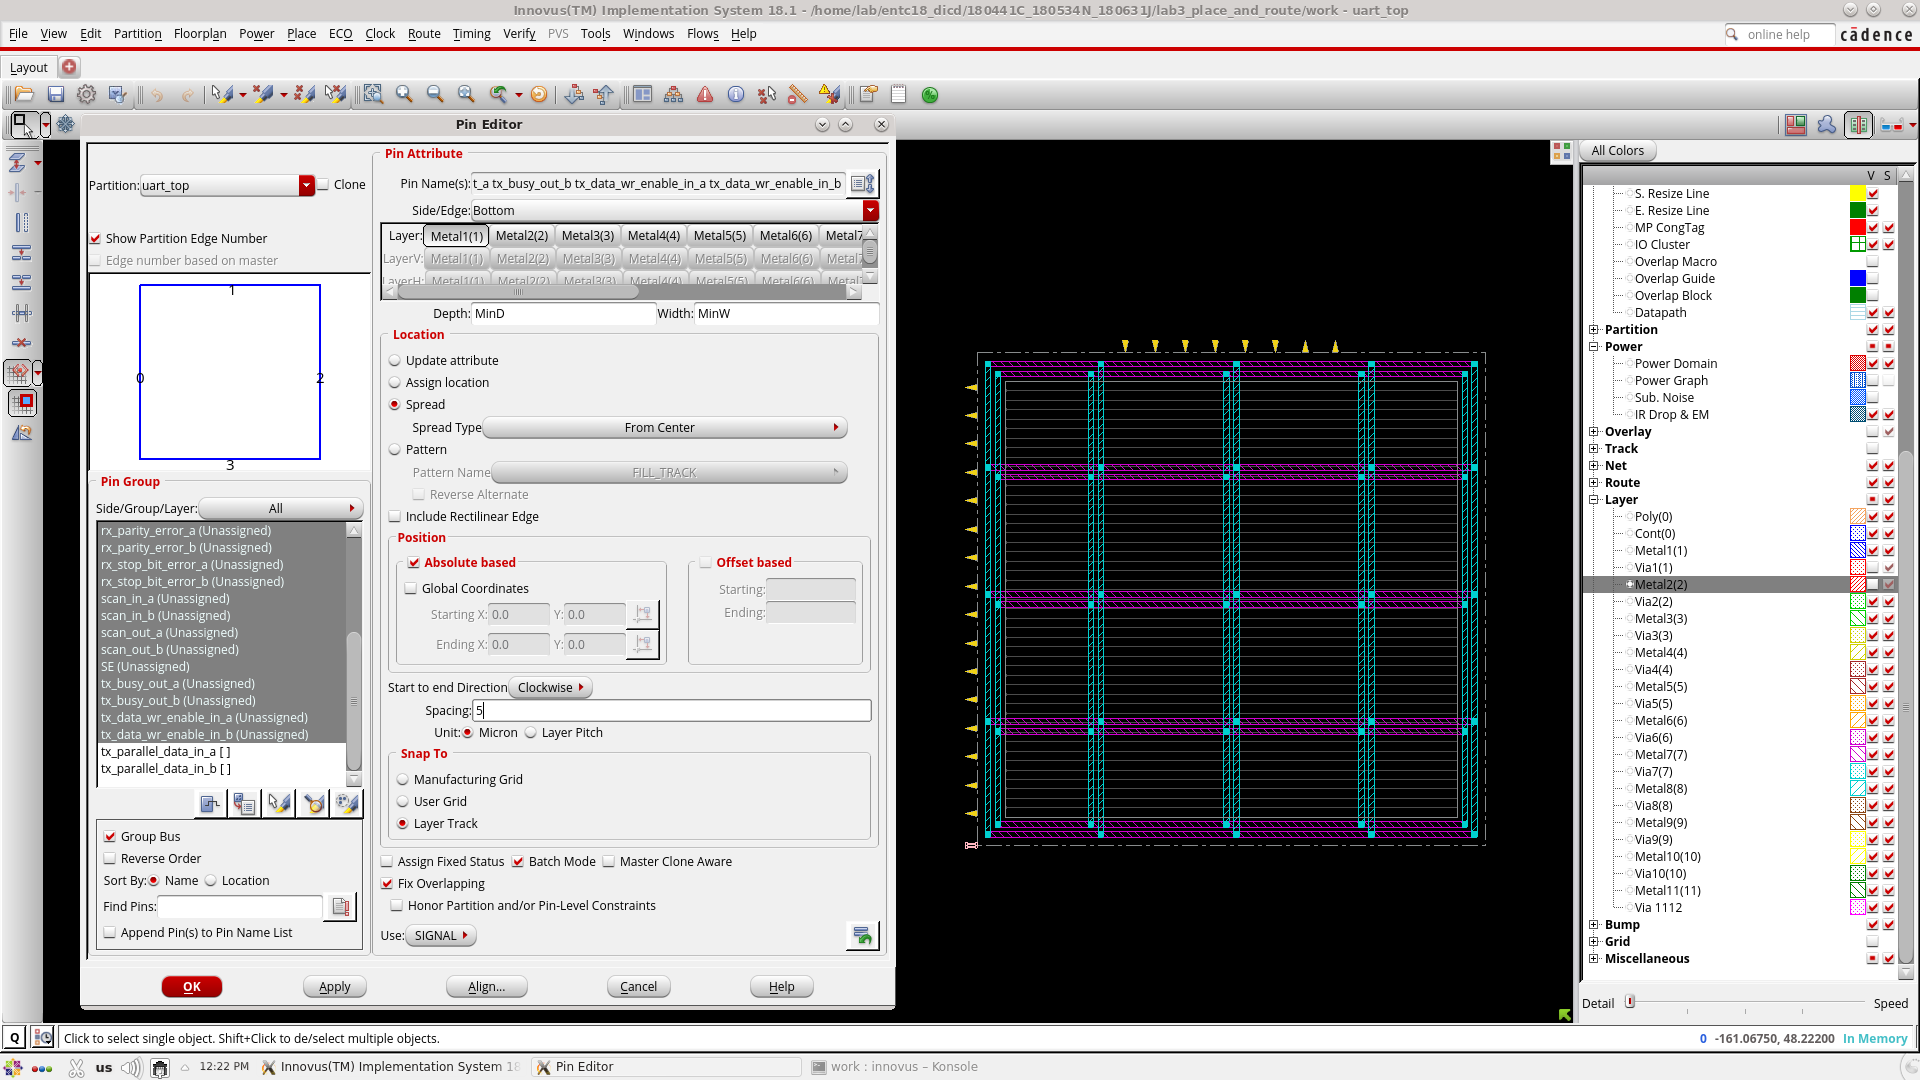
\includegraphics[width=0.9\linewidth]{figures/innovus_5_5.png}
		}
		\caption{Assigning the pins to the \ac{io} boundary}
		\label{fig:innovus_5_5}
	\end{figure}

	\begin{figure}[H]
		\centering
		\fbox{
			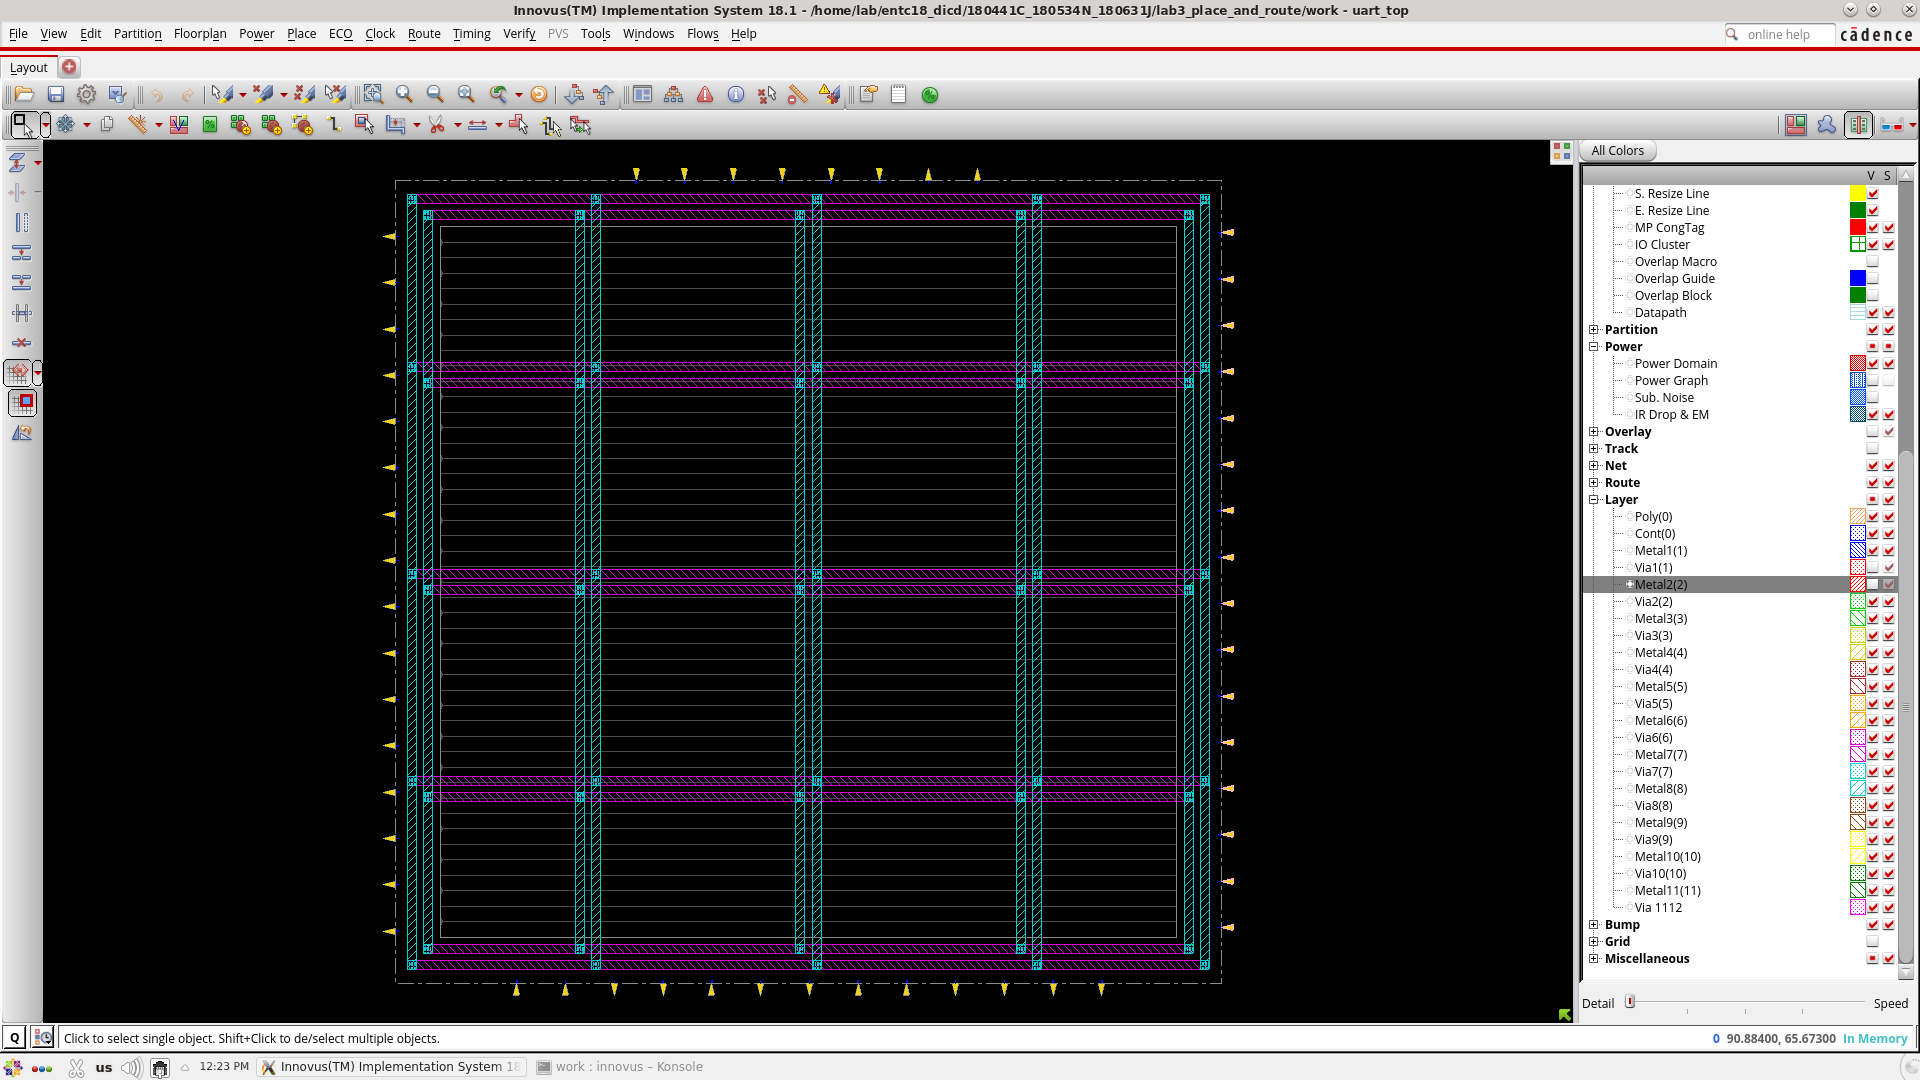
\includegraphics[width=0.9\linewidth]{figures/innovus_6_1.png}
		}
		\caption{View of the floorplan after the pins are assigned}
		\label{fig:innovus_6_1}
	\end{figure}
	
	\pagebreak
	\item Standard cell placement: this step runs a full placement with pre-place optimization as shown in the dialog box of the Figure \ref{fig:innovus_7_2}.
	
	\begin{figure}[H]
		\centering
		\fbox{
			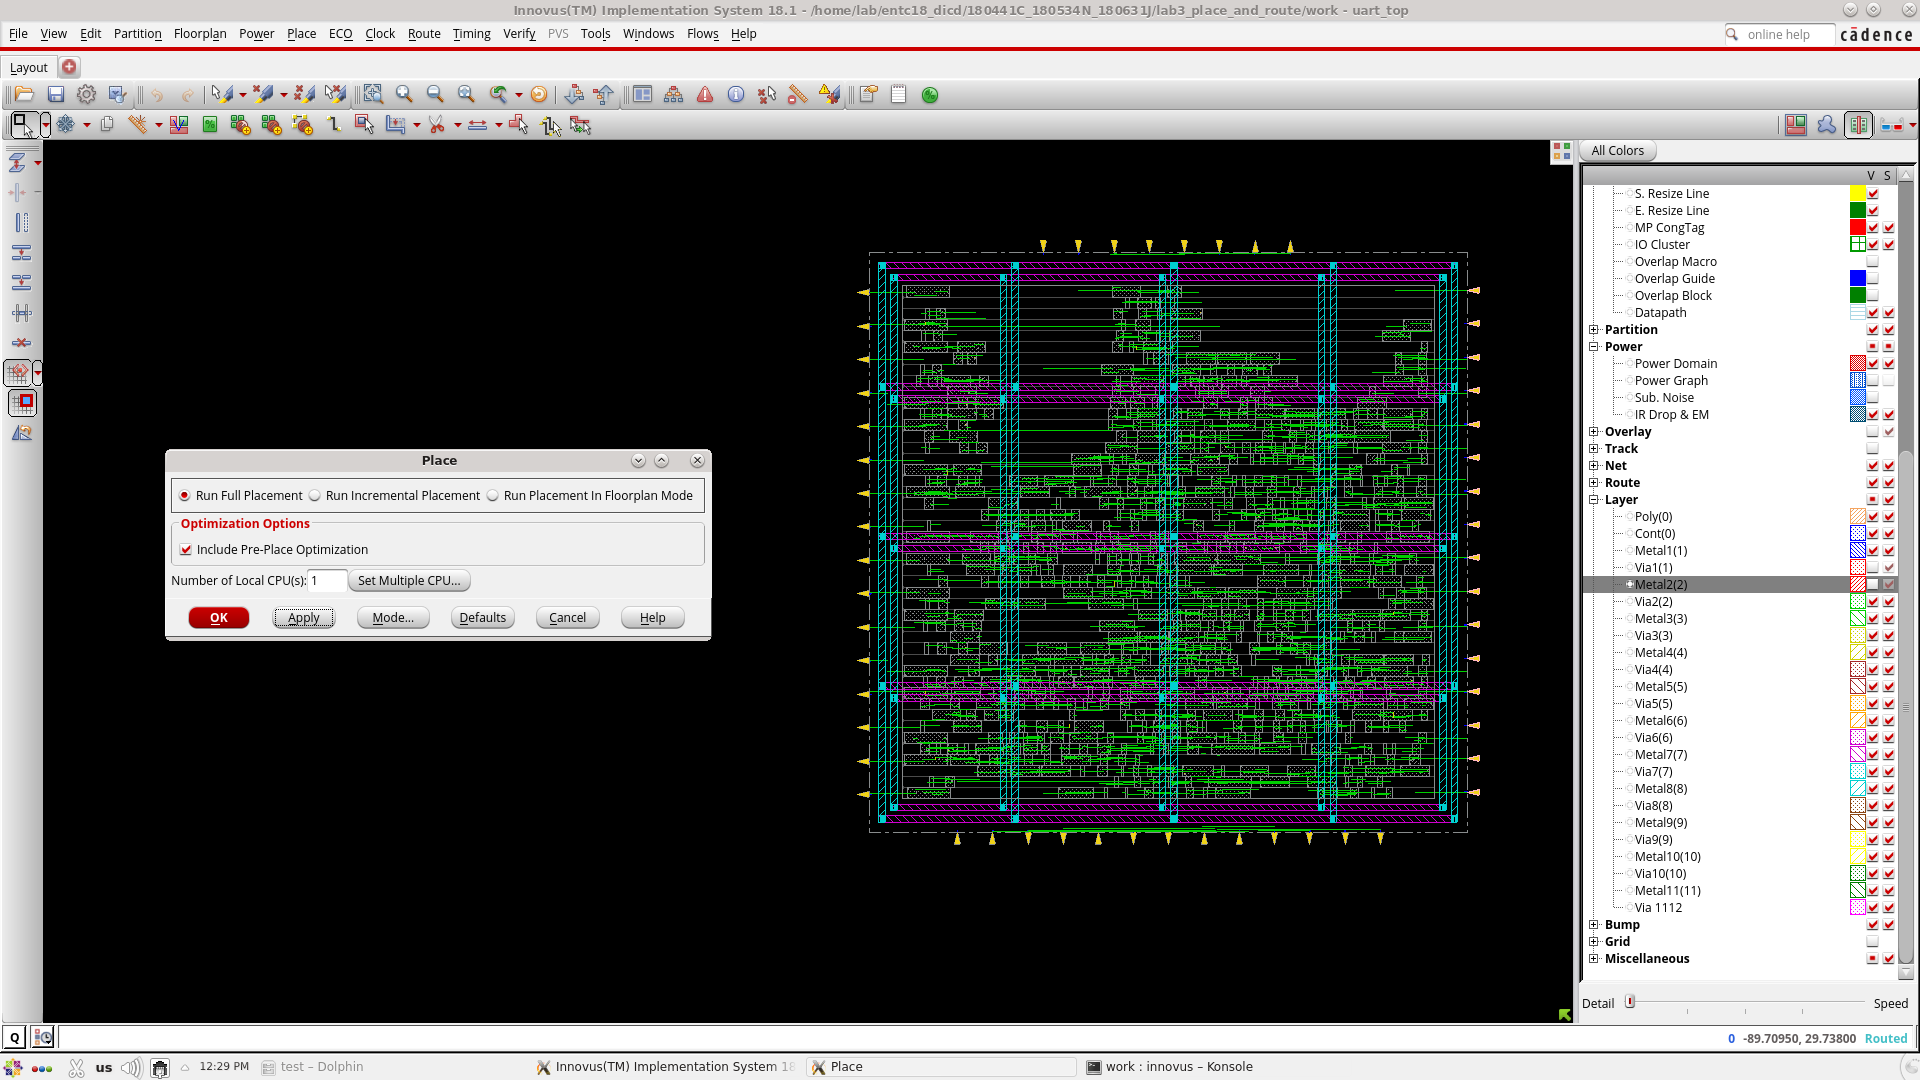
\includegraphics[width=0.9\linewidth]{figures/innovus_7_2.png}
		}
		\caption{`Run Full Placement' with `Pre-Place Optimization'}
		\label{fig:innovus_7_2}
	\end{figure}
	%TODO: check the validty of these ss. they are used in a ltare item!
	\begin{enumerate}[a.]
		\item A screenshot of the design without any nets
		\begin{figure}[H]
			\centering
			\fbox{
				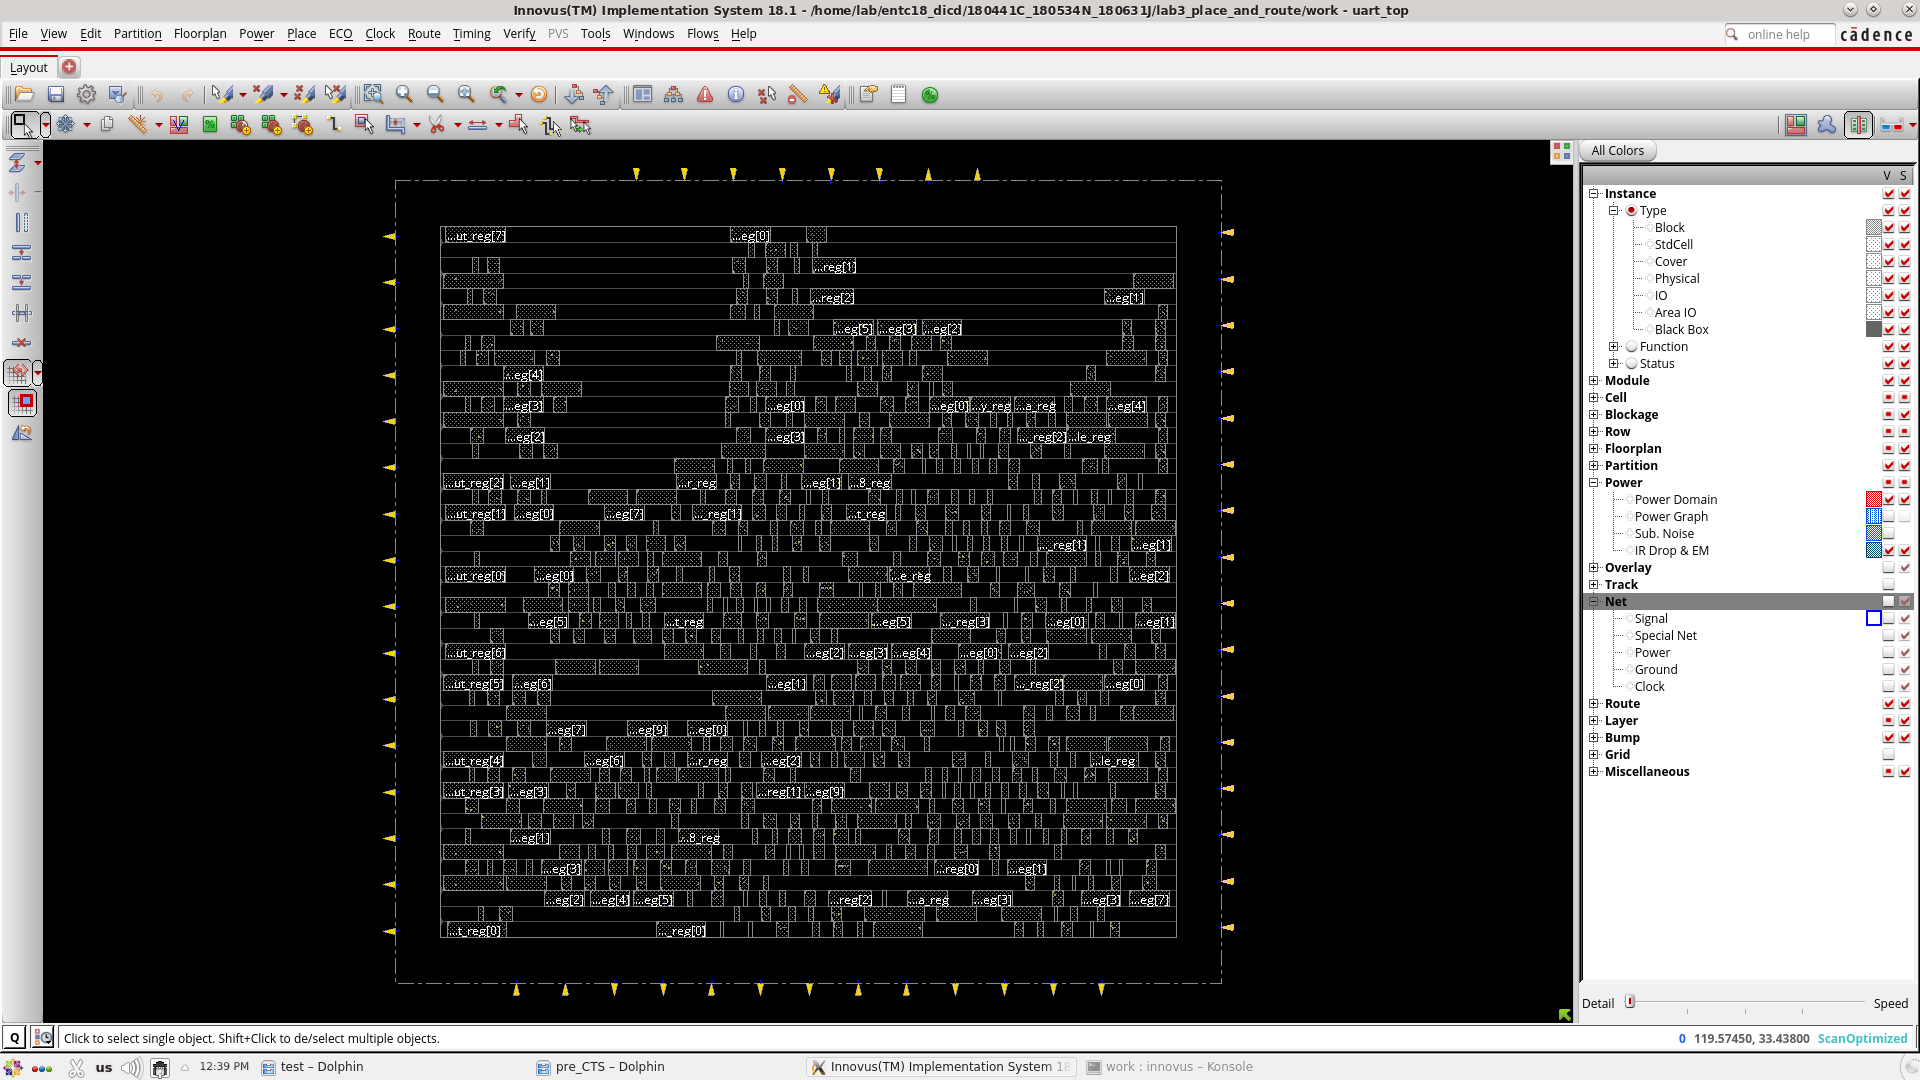
\includegraphics[width=0.9\linewidth]{figures/innovus_9_2.png}
			}
			\caption{Screenshot of the design without any nets}
			\label{fig:innovus_9_2}
		\end{figure}
		
		\item A screenshot of the design with the clock net		
		\begin{figure}[H]
			\centering
			\fbox{
				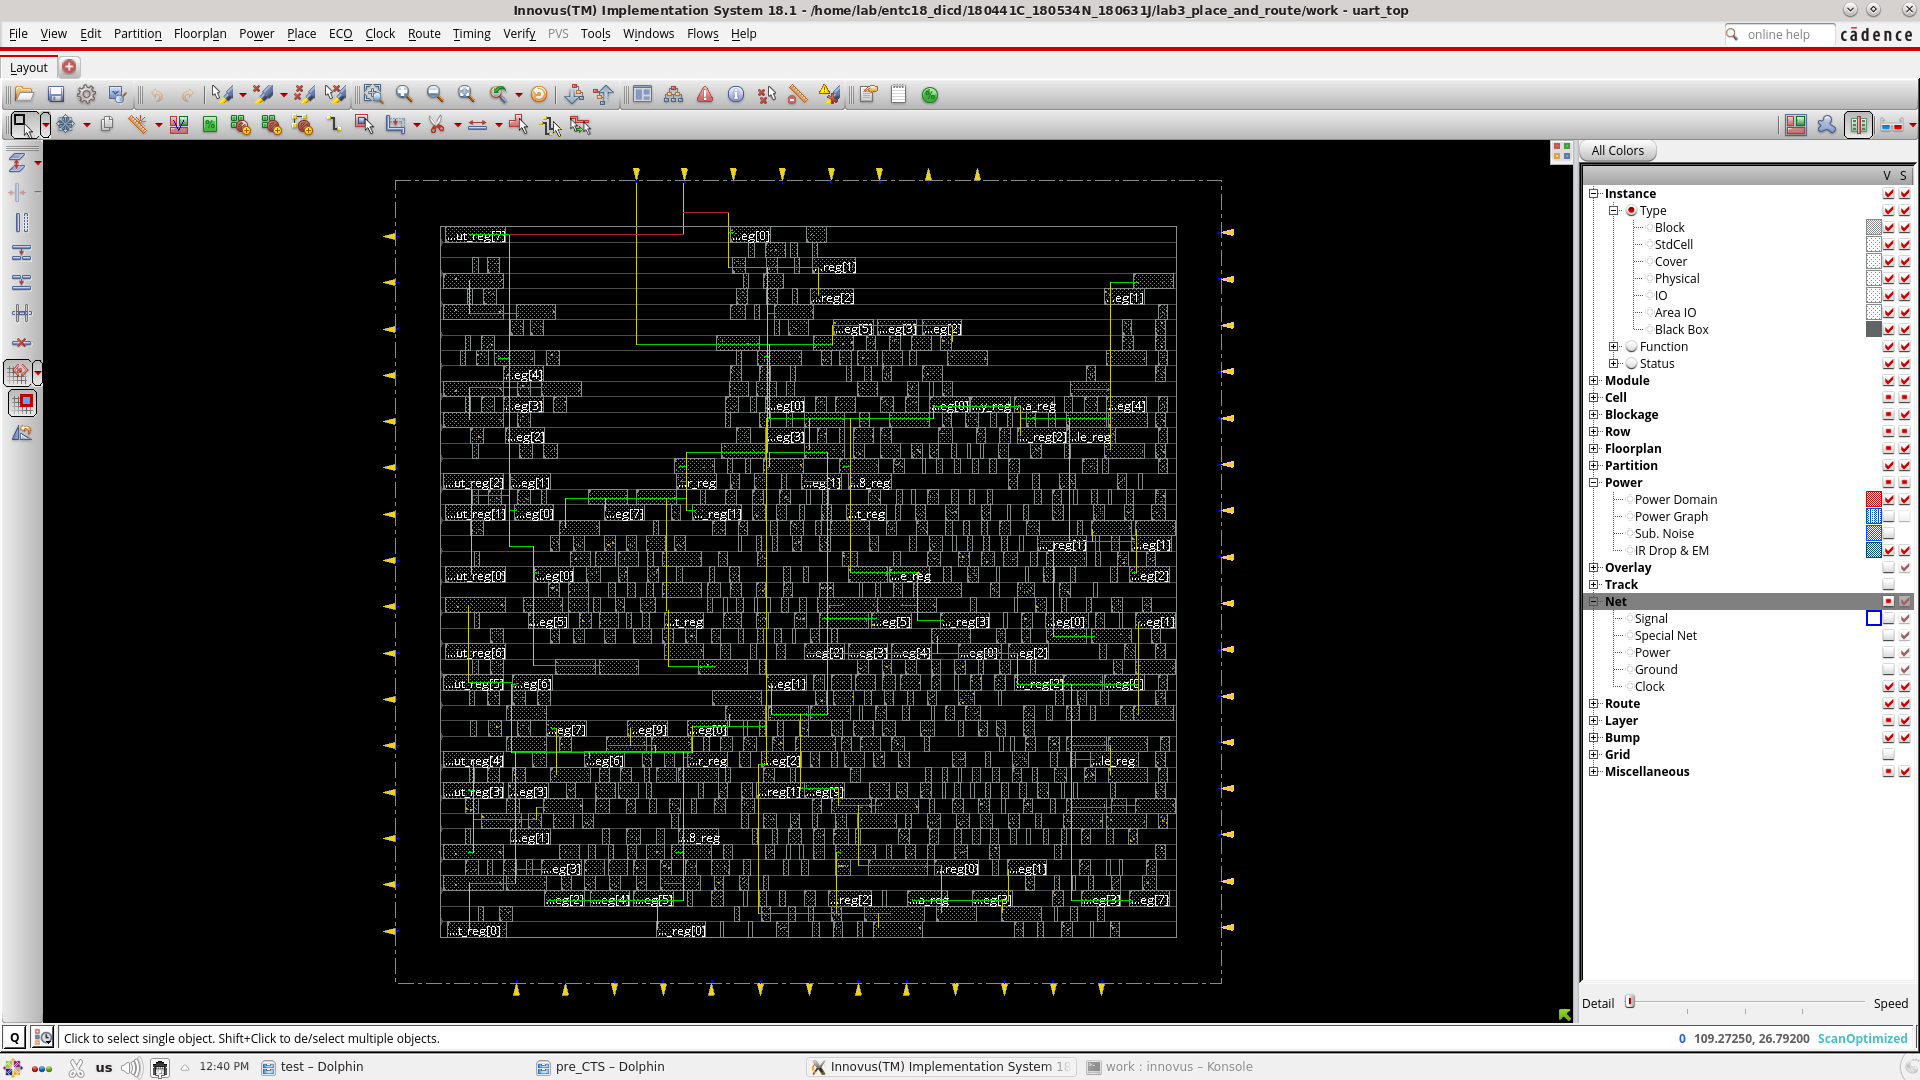
\includegraphics[width=0.9\linewidth]{figures/innovus_9_3.png}
			}
			\caption{Screenshot of the design with the clock net}
			\label{fig:innovus_9_3}
		\end{figure}
	\end{enumerate}
	
	\item  Report gate count and area
	\begin{figure}[H]
		\centering
		\fbox{
			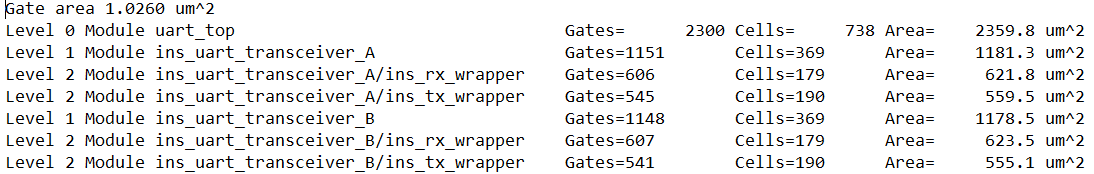
\includegraphics[width=0.9\linewidth]{figures/gateCount}
		}
		\caption{Gate count and the area report}
		\label{fig:gateCount}
	\end{figure}
	
	\item Pre-\ac{cts} setup time analysis: according to the given constraints,  there will be no violations at this stage. Summary of this is shown in the Figure \ref{fig:timeDesign}.
	
	\begin{figure}[H]
		\centering
		\fbox{
			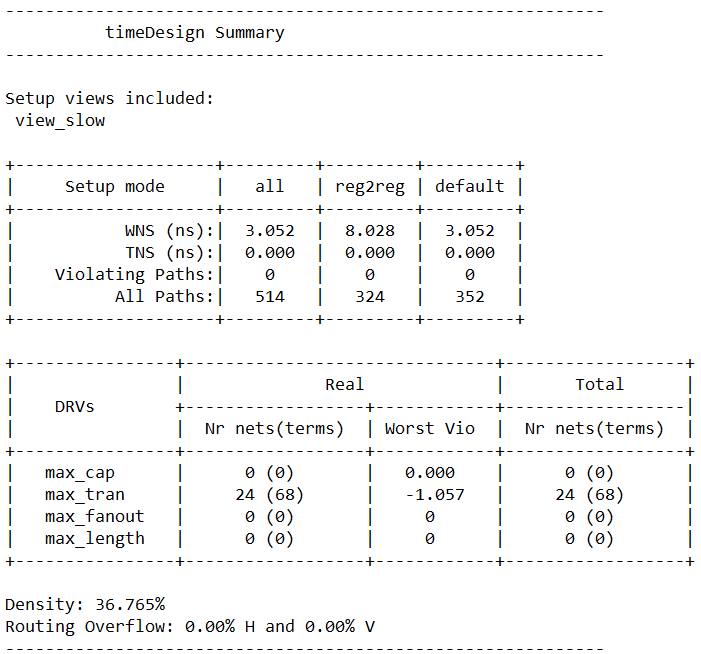
\includegraphics[width=0.6\linewidth]{figures/timeDesign }
		}
		\caption{Summary of the Pre-CTS setup time analysis}
		\label{fig:timeDesign}
	\end{figure} 
	
	
	\item Route power nets: observe the horizontal power routes spanning across the core area shown in the Figure \ref{fig:innovus_8_1}.
	\begin{figure}[H]
		\centering
		\fbox{
			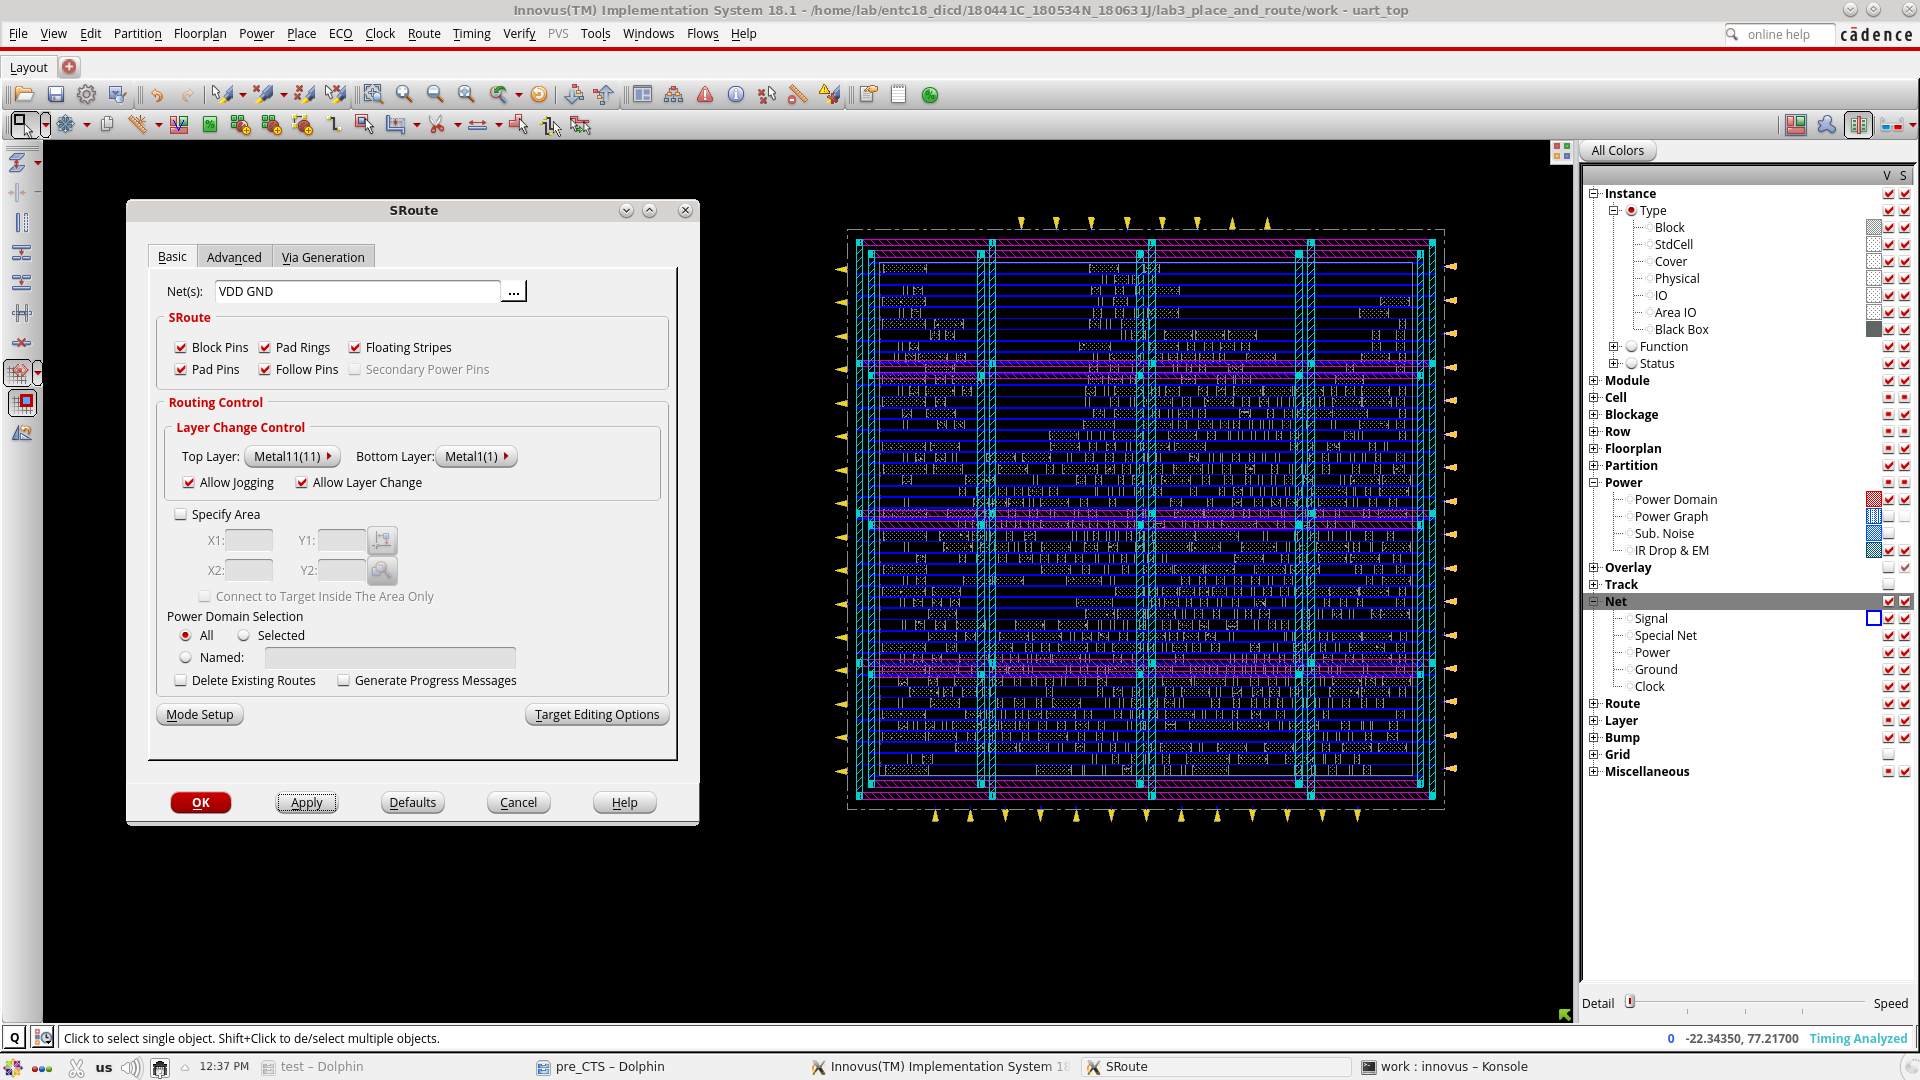
\includegraphics[width=0.9\linewidth]{figures/innovus_8_1.png}
		}
		\caption{Horizontal power routes spanning across the core area}
		\label{fig:innovus_8_1}
	\end{figure}

	\item \ac{cts} using {\tt ccopt\_design} command: resynthesize the clock net and add buffers or change wire lengths of clock nets to balance clock skew throughout the design.
	
	\begin{enumerate}[a.]
		\item A screenshot of the design without any nets after \ac{cts}
		\begin{figure}[H]
			\centering
			\fbox{
				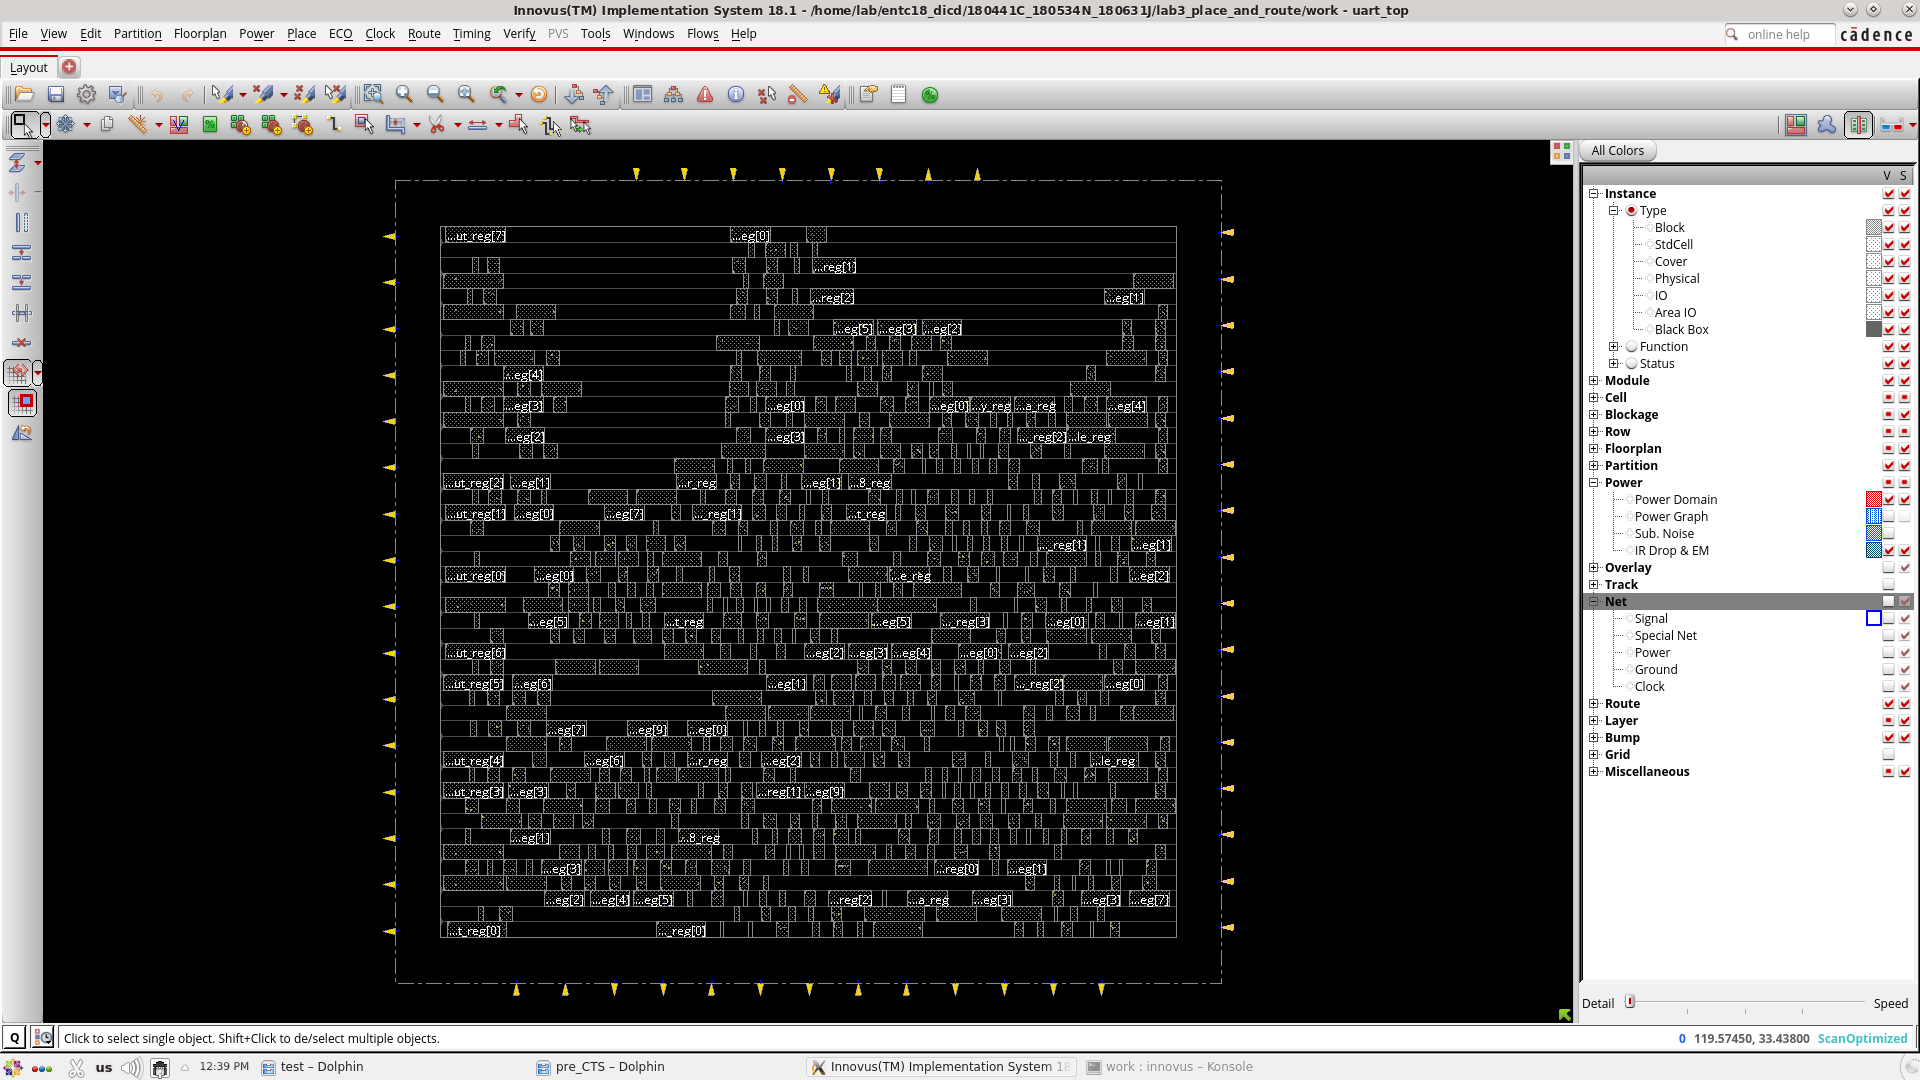
\includegraphics[width=0.9\linewidth]{figures/innovus_9_2.png}
			}
			\caption{Screenshot of the design without any nets after \ac{cts}}
			%\label{fig:innovus_9_2}
		\end{figure}
		
		\item A screenshot of the design with the clock net	after \ac{cts}	
		\begin{figure}[H]
			\centering
			\fbox{
				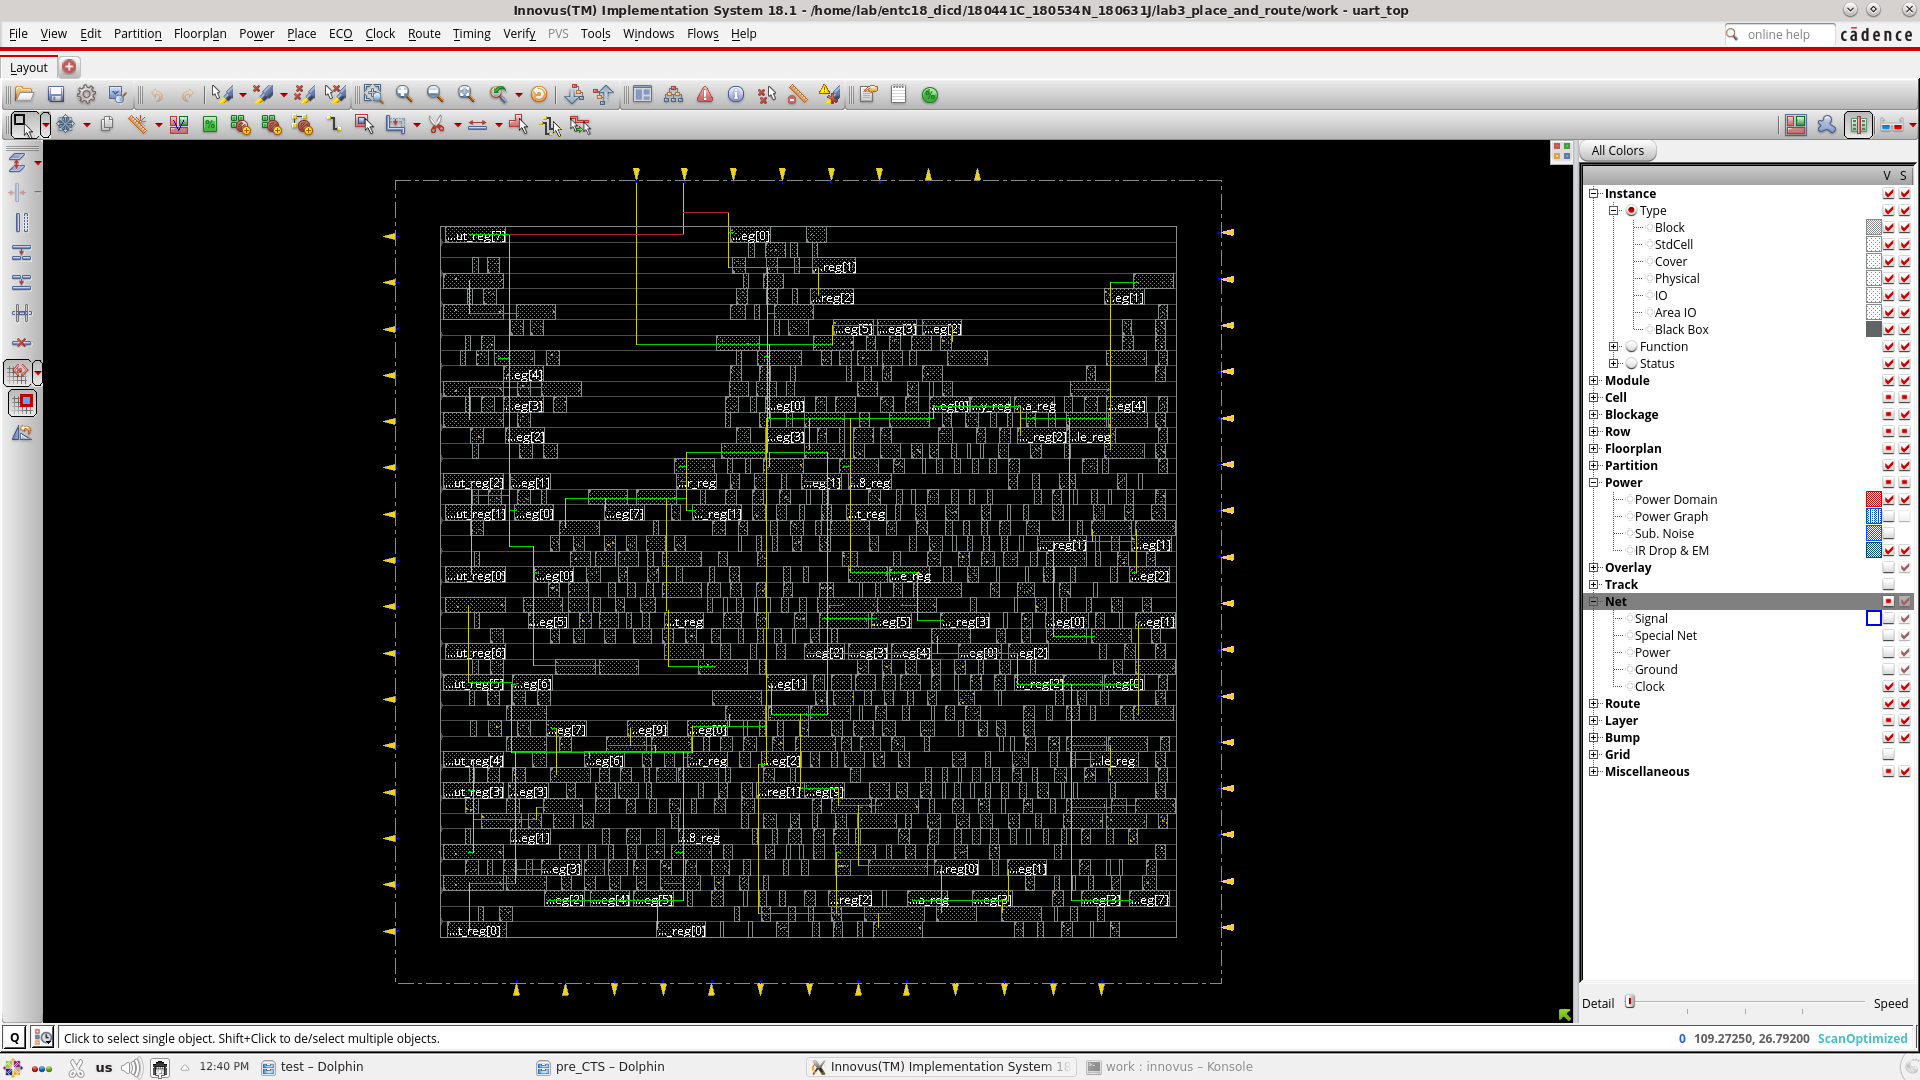
\includegraphics[width=0.9\linewidth]{figures/innovus_9_3.png}
			}
			\caption{Screenshot of the design with the clock net after \ac{cts}}
			%\label{fig:innovus_9_3}
		\end{figure}
	\end{enumerate}
	
	
\end{enumerate} 

\pagebreak
%\vfill
%\hrule
{\small
\bibliographystyle{IEEEtran}
\bibliography{refer}
}
%---------------------------------------------------------------------------
\end{document}
-
